\section{Vypracování}

Řešeným příkladem je známý \textit{Monty Hall Problem}.
V klasické verzi tohoto problému jsou stanoveny 3 předpoklady.

\begin{enumerate}
    \item Moderátor musí vybrat dveře, které nevybral soutěžící.
    \item Moderátor musí otevřít dveře, za kterými se ukrývá koza.
    \item Moderátor musí nabídnout soutěžícímu změnit vybrané dveře.
\end{enumerate}

\begin{figure}[htb]
    \centering
    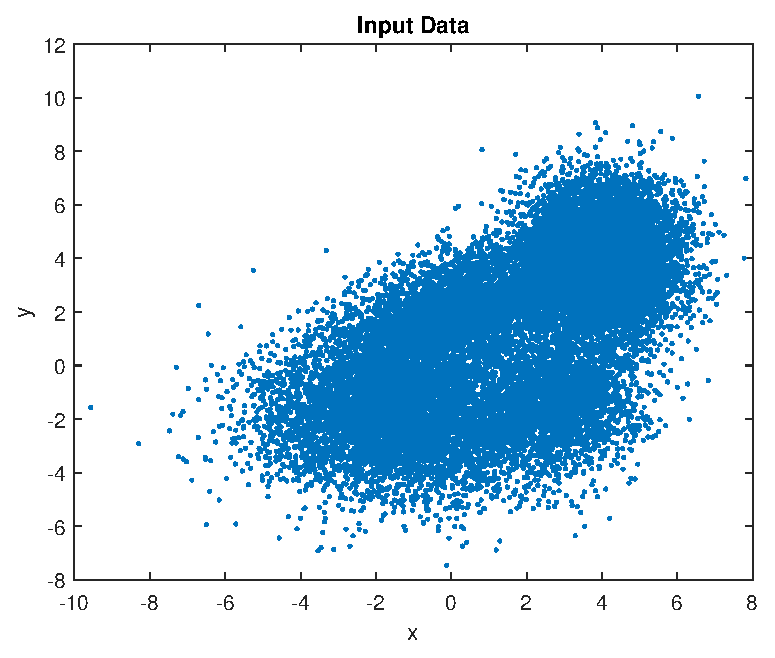
\includegraphics[width=0.55\textwidth]{graphs/fig1.eps}
    \caption{Závislost p-hodnoty oboustranného dvouvýběrového t-testu na velikosti souboru měření.}
    \label{fig:result1}
\end{figure}
\FloatBarrier

\begin{figure}[htb]
    \centering
    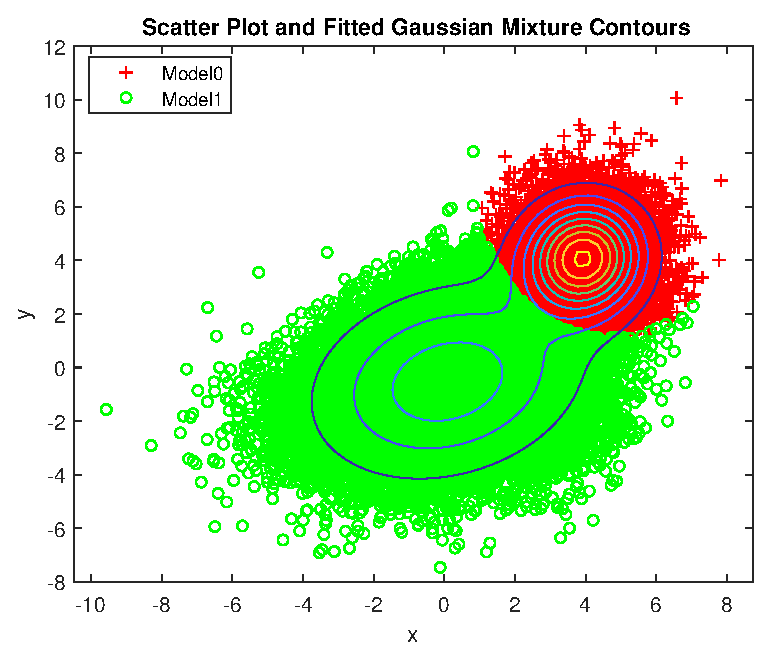
\includegraphics[width=0.55\textwidth]{graphs/fig2.eps}
    \caption{Závislost p-hodnoty oboustranného dvouvýběrového t-testu na velikosti souboru měření.}
    \label{fig:result2}
\end{figure}
\FloatBarrier

\begin{figure}[htb]
    \centering
    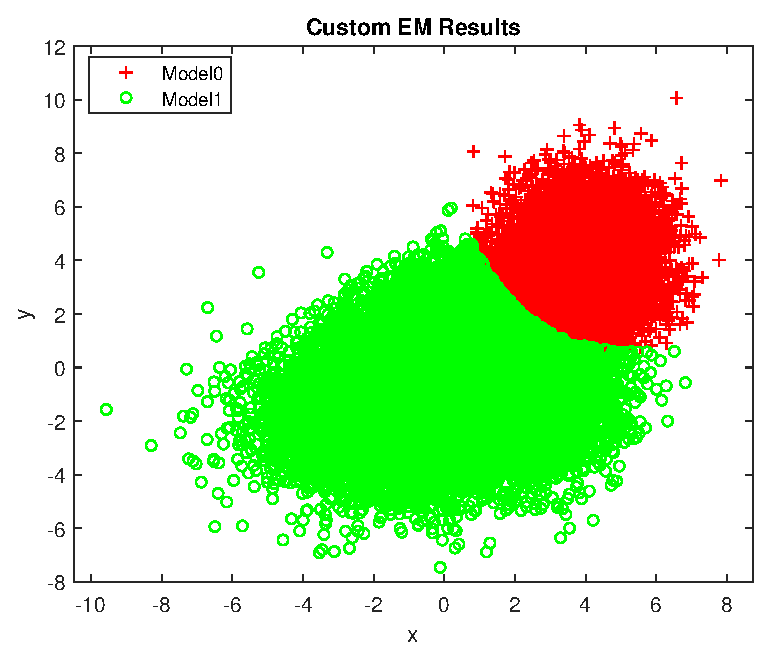
\includegraphics[width=0.55\textwidth]{graphs/fig3.eps}
    \caption{Závislost p-hodnoty oboustranného dvouvýběrového t-testu na velikosti souboru měření.}
    \label{fig:result3}
\end{figure}
\FloatBarrier

\begin{figure}[htb]
    \centering
    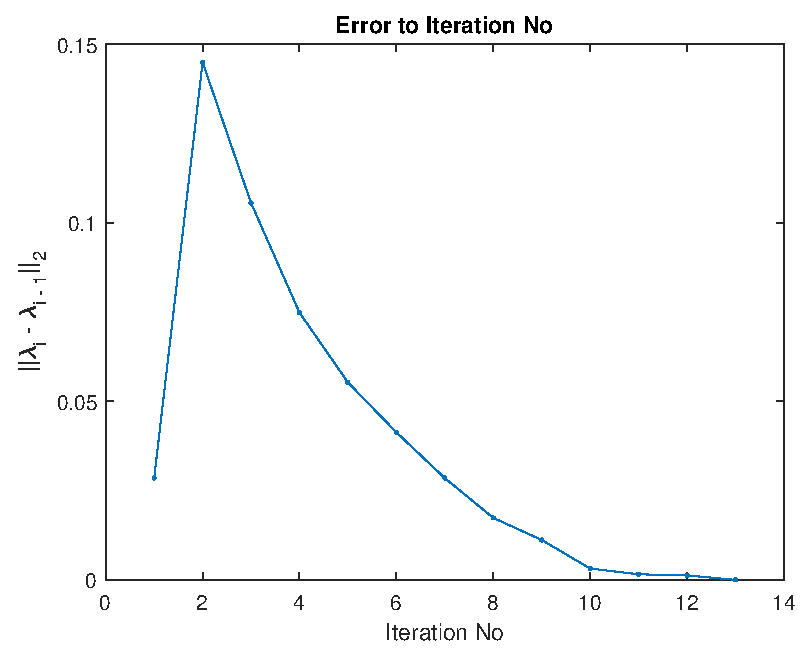
\includegraphics[width=0.55\textwidth]{graphs/fig4.eps}
    \caption{Závislost p-hodnoty oboustranného dvouvýběrového t-testu na velikosti souboru měření.}
    \label{fig:result4}
\end{figure}
\FloatBarrier

Řešení tohoto problému, ačkoliv možná neintuitivní, tak velice logické si lze snadno odvodit.
Představme si, že je nám dáno na výběr ze 100 dveří.
Za 99 dveřmi se ukrývají kozy a za právě jedněmi se ukrývá auto.
Náhodně vybereme jedny dveře, pravděpodobnost je tedy \( \frac{1}{100} \), že jsme vybrali dveře s autem.
Moderátor v následujícím kroku otevře 98 dveří, za kterými se ukrývají kozy.
Měly bychom změnit dveře?
Ano, měli bychom, protože pravděpodobnost, že jsme vybrali napoprvé správné dveře je velice malá.
Teď je nám ale prezentován filtrovaný výběr a mělo by být intuitivně jasné, že je pravděpodobnější, že se auto ukrývá za druhými dveřmi.
Takže pokud není naším cílem vyhrát kozu\ldots

\subsection{Matematika?}

Označme herní dveře \( i = \{0, 1, 2\}\) a výherní dveře \( D \).

\begin{equation}
    P(D = 0) = P(D = 1) = P(D = 2) = \frac{1}{3}
\end{equation}

Pozice výherních dveří je náhodná, v případě tří dveří je tedy pravděpodobnost jejich pozice jedna třetina.
Dveře vybrané hráčem označme jako \( C \).
\( C \) obecně není náhodné, učíme \( C = 0 \).
Hráč tedy vybral nulté dveře.
Posledním typem dveří je \( R \), dveře \enquote{odkryté} (\textit{revealed}).
Dle pravidel moderátor nesmí odkrýt dveře které vybral hráč \( R \neq C \) a nesmí vybrat dveře, kde se nachází auto \( R \neq D \).
Bez znalosti \( D \) můžeme napsat následující.

\begin{equation}
    P(R = 1) = P(R = 2) = \frac{1}{2}
\end{equation}

Řekněme, že \( R = 2 \), potom vyvstává otázka, jaká je pravděpodobnost, že \( D = 1 \).
Hledáme tedy \( P(D = 1 | R = 2) \).

\begin{align}
    P(D = 1 | R = 2) &= \frac{P(D = 1) \land P(R = 2)}{P(R = 2)} \\
    P(D = 1 | R = 2) &= \frac{P(R = 2 | D = 1) P(D = 1)}{P(R = 2)}
\end{align}

Protože \( P(D = 1) = \frac{1}{3} \), tak \( P(R = 2 | D = 1) \) musí být rovno jedné.
Někde \( R \) být musí a jelikož nemůže být na 0, protože to je hodnota zabraná hráčem a nemůže být na 1, protože to jsme právě stanovili na výherní dveře.

\begin{equation}
    P(D = 1 | R = 2) = \frac{1 \cdot \frac{1}{3}}{\frac{1}{2}} = \frac{2}{3}
\end{equation}

Pravděpodobnost, že se výherní dveře nacházejí za dveřmi \( D = 1 \) je tedy \( \frac{2}{3} \).
Obdobně můžeme postupovat pro problém čtyř dveří.

\section{Experimentální výsledky}

Tabulka~\ref{table:table1} znázorňuje experimentální výsledky pro problém tří dveří.

\begin{table}[htb]
    \centering

    \begin{tabular}{ccc}
        \toprule

        Změna hráčem    & Moderátor volí náhodně    & Moderátor volí nevýherní dveře    \\ \midrule
        Ne              & 0.3322                    & 0.3339                            \\
        Ano             & 0.3324                    & 0.6661                            \\
          
        \bottomrule
    \end{tabular}

    \caption{Výsledné hodnoty pravděpodobností pro MHP 3 dveře pro 100.000 odsimulovaných her}
    \label{table:table1}
\end{table}
\FloatBarrier

Tabulka~\ref{table:table2} znázorňuje experimentální výsledky pro problém čtyř dveří.

\begin{table}[htb]
    \centering

    \begin{tabular}{cccc}
        \toprule

        Změna hráčem 1  & Změna hráčem 2    & Moderátor volí náhodně    & Moderátor volí nevýherní dveře    \\ \midrule
        Ano             & Ano               & 0.1403                    & 0.6248                            \\
        Ne              & Ano               & 0.1380                    & 0.7509                            \\
        Ano             & Ne                & 0.2530                    & 0.3734                            \\
        Ne              & Ne                & 0.2485                    & 0.2513                            \\

        \bottomrule
    \end{tabular}

    \caption{Výsledné hodnoty pravděpodobností pro MHP 4 dveře pro 100.000 odsimulovaných her}
    \label{table:table2}
\end{table}
\FloatBarrier

\section{Závěr}

Experimentální výsledky potvrzují teorii.
V případě, že moderátor volí náhodně, tak je prakticky jedno co hráč udělá, pravděpodobnost výhry je rovna náhodnému výběru.
V případě, že moderátor otevírá pouze nevýherní dveře, je pravděpodobnost dle teorie rovna \( 66 \: \% \), v případě čtyř dveří ekvivalentně \( 75 \: \% \).
